\documentclass{standalone}
\usepackage{tikz}
\usetikzlibrary{patterns, positioning}
\usepackage[sfdefault]{ClearSans} %% option 'sfdefault' activates Clear Sans as the default text font
\usepackage[T1]{fontenc}

\begin{document}
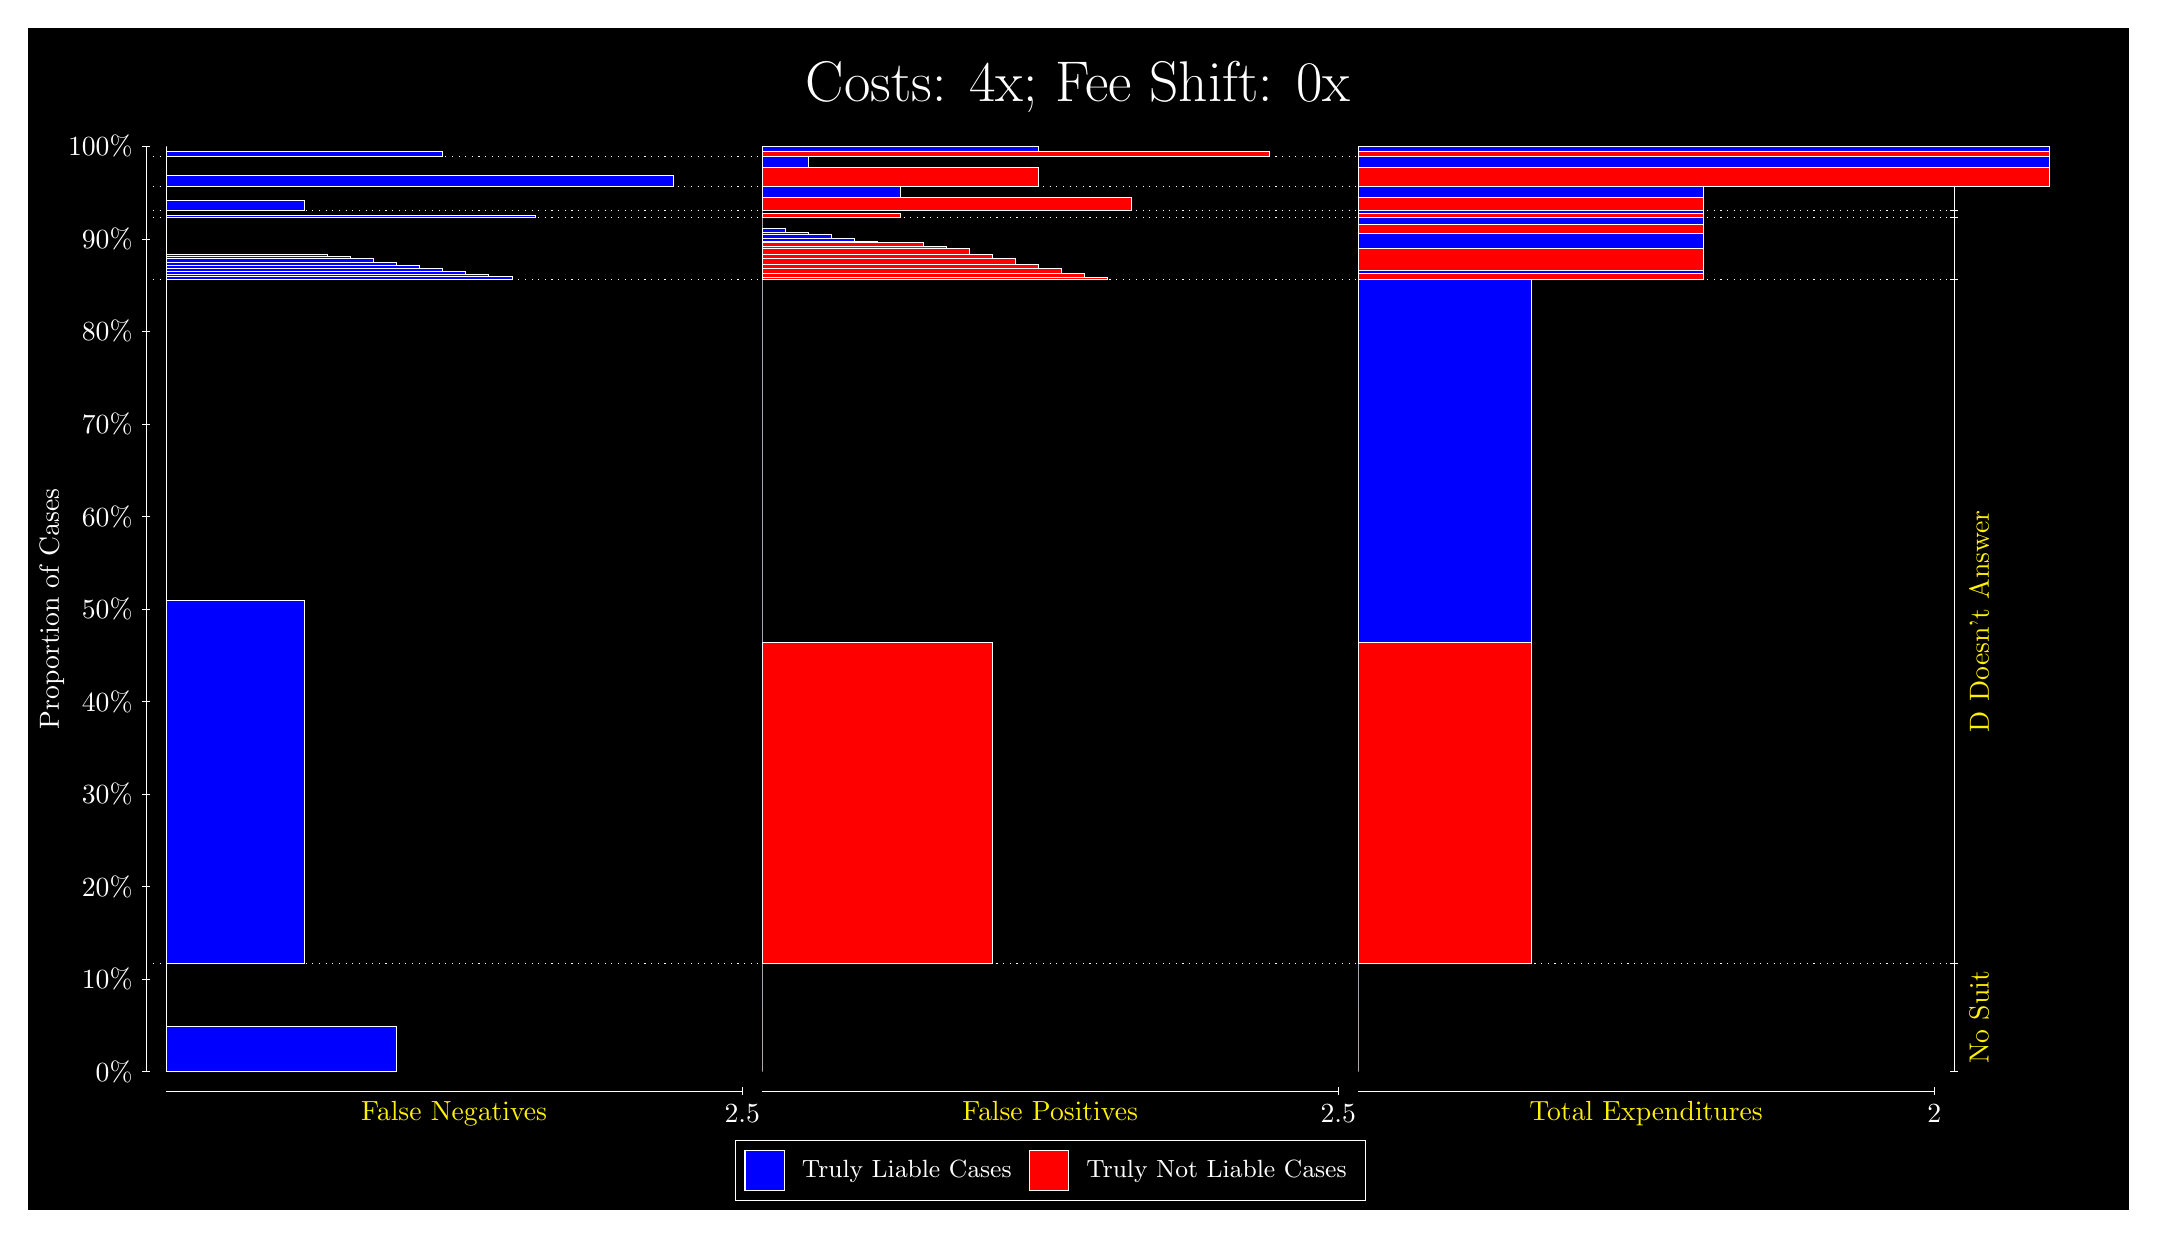
\begin{tikzpicture}
\draw[fill=black] (0,0) rectangle (26.667,15);
\draw[text=white] (0,13.5) rectangle (26.667,15) node[midway] {\huge Costs: 4x; Fee Shift: 0x};
\draw[white, very thin] (1.5,1.75) -- (1.5,13.5);
\node[rotate=90, text=white, anchor=center] at (0.3, 7.625) {Proportion of Cases};
\draw[white, very thin] (1.45,1.75) -- (1.55,1.75);
\node[text=white, anchor=east] at (1.45, 1.75) {0\%};
\draw[white, very thin] (1.45,2.925) -- (1.55,2.925);
\node[text=white, anchor=east] at (1.45, 2.925) {10\%};
\draw[white, very thin] (1.45,4.1) -- (1.55,4.1);
\node[text=white, anchor=east] at (1.45, 4.1) {20\%};
\draw[white, very thin] (1.45,5.275) -- (1.55,5.275);
\node[text=white, anchor=east] at (1.45, 5.275) {30\%};
\draw[white, very thin] (1.45,6.45) -- (1.55,6.45);
\node[text=white, anchor=east] at (1.45, 6.45) {40\%};
\draw[white, very thin] (1.45,7.625) -- (1.55,7.625);
\node[text=white, anchor=east] at (1.45, 7.625) {50\%};
\draw[white, very thin] (1.45,8.8) -- (1.55,8.8);
\node[text=white, anchor=east] at (1.45, 8.8) {60\%};
\draw[white, very thin] (1.45,9.975) -- (1.55,9.975);
\node[text=white, anchor=east] at (1.45, 9.975) {70\%};
\draw[white, very thin] (1.45,11.15) -- (1.55,11.15);
\node[text=white, anchor=east] at (1.45, 11.15) {80\%};
\draw[white, very thin] (1.45,12.325) -- (1.55,12.325);
\node[text=white, anchor=east] at (1.45, 12.325) {90\%};
\draw[white, very thin] (1.45,13.5) -- (1.55,13.5);
\node[text=white, anchor=east] at (1.45, 13.5) {100\%};

\draw[white, very thin] (24.457,1.75) -- (24.457,13.5);
\draw[white, very thin] (24.407,1.75) -- (24.507,1.75);
\node[anchor=west] at (24.407, 1.75) {};
\draw[white, very thin] (24.407,3.1251) -- (24.507,3.1251);
\node[anchor=west] at (24.407, 3.1251) {};
\draw[white, very thin] (24.407,11.813) -- (24.507,11.813);
\node[anchor=west] at (24.407, 11.813) {};
\draw[white, very thin] (24.407,12.594) -- (24.507,12.594);
\node[anchor=west] at (24.407, 12.594) {};
\draw[white, very thin] (24.407,12.689) -- (24.507,12.689);
\node[anchor=west] at (24.407, 12.689) {};
\draw[white, very thin] (24.407,12.992) -- (24.507,12.992);
\node[anchor=west] at (24.407, 12.992) {};
\draw[white, very thin] (24.407,13.372) -- (24.507,13.372);
\node[anchor=west] at (24.407, 13.372) {};
\draw[white, very thin] (24.407,13.5) -- (24.507,13.5);
\node[anchor=west] at (24.407, 13.5) {};

\draw[white, very thin, fill=blue] (1.75,1.75) rectangle (4.6775,2.3198);
\draw[white, very thin, fill=red] (1.75,2.3198) rectangle (1.75,3.1251);
\draw[white, very thin, fill=blue] (1.75,3.1251) rectangle (3.5065,7.7395);
\draw[white, very thin, fill=red] (1.75,7.7395) rectangle (1.75,11.813);
\draw[white, very thin, fill=blue] (1.75,11.813) rectangle (6.1413,11.844);
\draw[white, very thin, fill=blue] (1.75,11.844) rectangle (5.8486,11.869);
\draw[white, very thin, fill=blue] (1.75,11.869) rectangle (5.5558,11.916);
\draw[white, very thin, fill=blue] (1.75,11.916) rectangle (5.2631,11.948);
\draw[white, very thin, fill=blue] (1.75,11.948) rectangle (4.9703,11.995);
\draw[white, very thin, fill=blue] (1.75,11.995) rectangle (4.6775,12.027);
\draw[white, very thin, fill=blue] (1.75,12.027) rectangle (4.3848,12.075);
\draw[white, very thin, fill=blue] (1.75,12.075) rectangle (4.092,12.109);
\draw[white, very thin, fill=blue] (1.75,12.109) rectangle (3.7993,12.129);
\draw[white, very thin, fill=red] (1.75,12.129) rectangle (1.75,12.594);
\draw[white, very thin, fill=blue] (1.75,12.594) rectangle (6.4341,12.629);
\draw[white, very thin, fill=red] (1.75,12.629) rectangle (1.75,12.689);
\draw[white, very thin, fill=blue] (1.75,12.689) rectangle (3.5065,12.821);
\draw[white, very thin, fill=red] (1.75,12.821) rectangle (1.75,12.992);
\draw[white, very thin, fill=blue] (1.75,12.992) rectangle (8.1906,13.132);
\draw[white, very thin, fill=red] (1.75,13.132) rectangle (1.75,13.372);
\draw[white, very thin, fill=blue] (1.75,13.372) rectangle (5.2631,13.438);
\draw[white, very thin, fill=red] (1.75,13.438) rectangle (1.75,13.5);
\draw[white, very thin, fill=red] (9.3189,1.75) rectangle (9.3189,2.5553);
\draw[white, very thin, fill=blue] (9.3189,2.5553) rectangle (9.3189,3.1251);
\draw[white, very thin, fill=red] (9.3189,3.1251) rectangle (12.246,7.1987);
\draw[white, very thin, fill=blue] (9.3189,7.1987) rectangle (9.3189,11.813);
\draw[white, very thin, fill=red] (9.3189,11.813) rectangle (13.71,11.837);
\draw[white, very thin, fill=red] (9.3189,11.837) rectangle (13.417,11.882);
\draw[white, very thin, fill=red] (9.3189,11.882) rectangle (13.125,11.952);
\draw[white, very thin, fill=red] (9.3189,11.952) rectangle (12.832,12.005);
\draw[white, very thin, fill=red] (9.3189,12.005) rectangle (12.539,12.078);
\draw[white, very thin, fill=red] (9.3189,12.078) rectangle (12.246,12.126);
\draw[white, very thin, fill=red] (9.3189,12.126) rectangle (11.954,12.2);
\draw[white, very thin, fill=red] (9.3189,12.2) rectangle (11.661,12.235);
\draw[white, very thin, fill=red] (9.3189,12.235) rectangle (11.368,12.278);
\draw[white, very thin, fill=blue] (9.3189,12.278) rectangle (10.783,12.298);
\draw[white, very thin, fill=blue] (9.3189,12.298) rectangle (10.49,12.332);
\draw[white, very thin, fill=blue] (9.3189,12.332) rectangle (10.197,12.38);
\draw[white, very thin, fill=blue] (9.3189,12.38) rectangle (9.9044,12.412);
\draw[white, very thin, fill=blue] (9.3189,12.412) rectangle (9.6116,12.459);
\draw[white, very thin, fill=blue] (9.3189,12.459) rectangle (9.3189,12.594);
\draw[white, very thin, fill=red] (9.3189,12.594) rectangle (11.075,12.653);
\draw[white, very thin, fill=blue] (9.3189,12.653) rectangle (9.3189,12.689);
\draw[white, very thin, fill=red] (9.3189,12.689) rectangle (14.003,12.859);
\draw[white, very thin, fill=blue] (9.3189,12.859) rectangle (11.075,12.992);
\draw[white, very thin, fill=red] (9.3189,12.992) rectangle (12.832,13.231);
\draw[white, very thin, fill=blue] (9.3189,13.231) rectangle (9.9044,13.372);
\draw[white, very thin, fill=red] (9.3189,13.372) rectangle (15.759,13.434);
\draw[white, very thin, fill=blue] (9.3189,13.434) rectangle (12.832,13.5);
\draw[white, very thin, fill=red] (16.888,1.75) rectangle (16.888,2.5553);
\draw[white, very thin, fill=blue] (16.888,2.5553) rectangle (16.888,3.1251);
\draw[white, very thin, fill=red] (16.888,3.1251) rectangle (19.083,7.1987);
\draw[white, very thin, fill=blue] (16.888,7.1987) rectangle (19.083,11.813);
\draw[white, very thin, fill=red] (16.888,11.813) rectangle (21.279,11.886);
\draw[white, very thin, fill=blue] (16.888,11.886) rectangle (21.279,11.932);
\draw[white, very thin, fill=red] (16.888,11.932) rectangle (21.279,12.21);
\draw[white, very thin, fill=blue] (16.888,12.21) rectangle (21.279,12.397);
\draw[white, very thin, fill=red] (16.888,12.397) rectangle (21.279,12.512);
\draw[white, very thin, fill=blue] (16.888,12.512) rectangle (21.279,12.594);
\draw[white, very thin, fill=red] (16.888,12.594) rectangle (21.279,12.653);
\draw[white, very thin, fill=blue] (16.888,12.653) rectangle (21.279,12.689);
\draw[white, very thin, fill=red] (16.888,12.689) rectangle (21.279,12.859);
\draw[white, very thin, fill=blue] (16.888,12.859) rectangle (21.279,12.992);
\draw[white, very thin, fill=red] (16.888,12.992) rectangle (25.67,13.231);
\draw[white, very thin, fill=blue] (16.888,13.231) rectangle (25.67,13.372);
\draw[white, very thin, fill=red] (16.888,13.372) rectangle (25.67,13.434);
\draw[white, very thin, fill=blue] (16.888,13.434) rectangle (25.67,13.5);
\draw[white, dotted] (1.5,3.1251) -- (24.457,3.1251);
\draw[white, dotted] (1.5,11.813) -- (24.457,11.813);
\draw[white, dotted] (1.5,12.594) -- (24.457,12.594);
\draw[white, dotted] (1.5,12.689) -- (24.457,12.689);
\draw[white, dotted] (1.5,12.992) -- (24.457,12.992);
\draw[white, dotted] (1.5,13.372) -- (24.457,13.372);
\draw[white, very thin] (1.75,1.5) -- (9.0689,1.5);
\node[text=yellow, anchor=north] at (5.4094, 1.5) {False Negatives};
\draw[white, very thin] (9.0689,1.45) -- (9.0689,1.55);
\node[text=white, anchor=north] at (9.0689, 1.45) {2.5};

\draw[white, very thin] (9.3189,1.5) -- (16.638,1.5);
\node[text=yellow, anchor=north] at (12.978, 1.5) {False Positives};
\draw[white, very thin] (16.638,1.45) -- (16.638,1.55);
\node[text=white, anchor=north] at (16.638, 1.45) {2.5};

\draw[white, very thin] (16.888,1.5) -- (24.207,1.5);
\node[text=yellow, anchor=north] at (20.547, 1.5) {Total Expenditures};
\draw[white, very thin] (24.207,1.45) -- (24.207,1.55);
\node[text=white, anchor=north] at (24.207, 1.45) {2};

\node[text=yellow, centered, rotate=90] at (24.777, 2.4376) {No Suit};
\node[text=yellow, centered, rotate=90] at (24.777, 7.4691) {D Doesn't Answer};






\draw (12.978300999999998,1.5) node[draw=none] (baseCoordinate) {};
\begin{scope}[align=center]
        \matrix[scale=0.5, draw=white, below=0.5cm of baseCoordinate, nodes={draw}, column sep=0.1cm]{
            \node[rectangle, draw, minimum width=0.5cm, minimum height=0.5cm, fill=blue] {}; &
            \node[draw=none, font=\small, text=white] (B) {Truly Liable Cases}; &
            \node[rectangle, draw, minimum width=0.5cm, minimum height=0.5cm, fill=red] {}; &
            \node[draw=none, font=\small, text=white] (B) {Truly Not Liable Cases}; \\
            };
\end{scope}

\end{tikzpicture}
\end{document}